\chapter{Results and Discussions}\label{Chapter:results}

\section{Lookup Tables}

\begin{figure}[ht] 
	\begin{subfigure}[b]{0.5\linewidth}
		\centering
		\ifpdf
		\includegraphics[width=0.95\linewidth]{./figs/lookup/baseline-loss-pdf}
		\else
		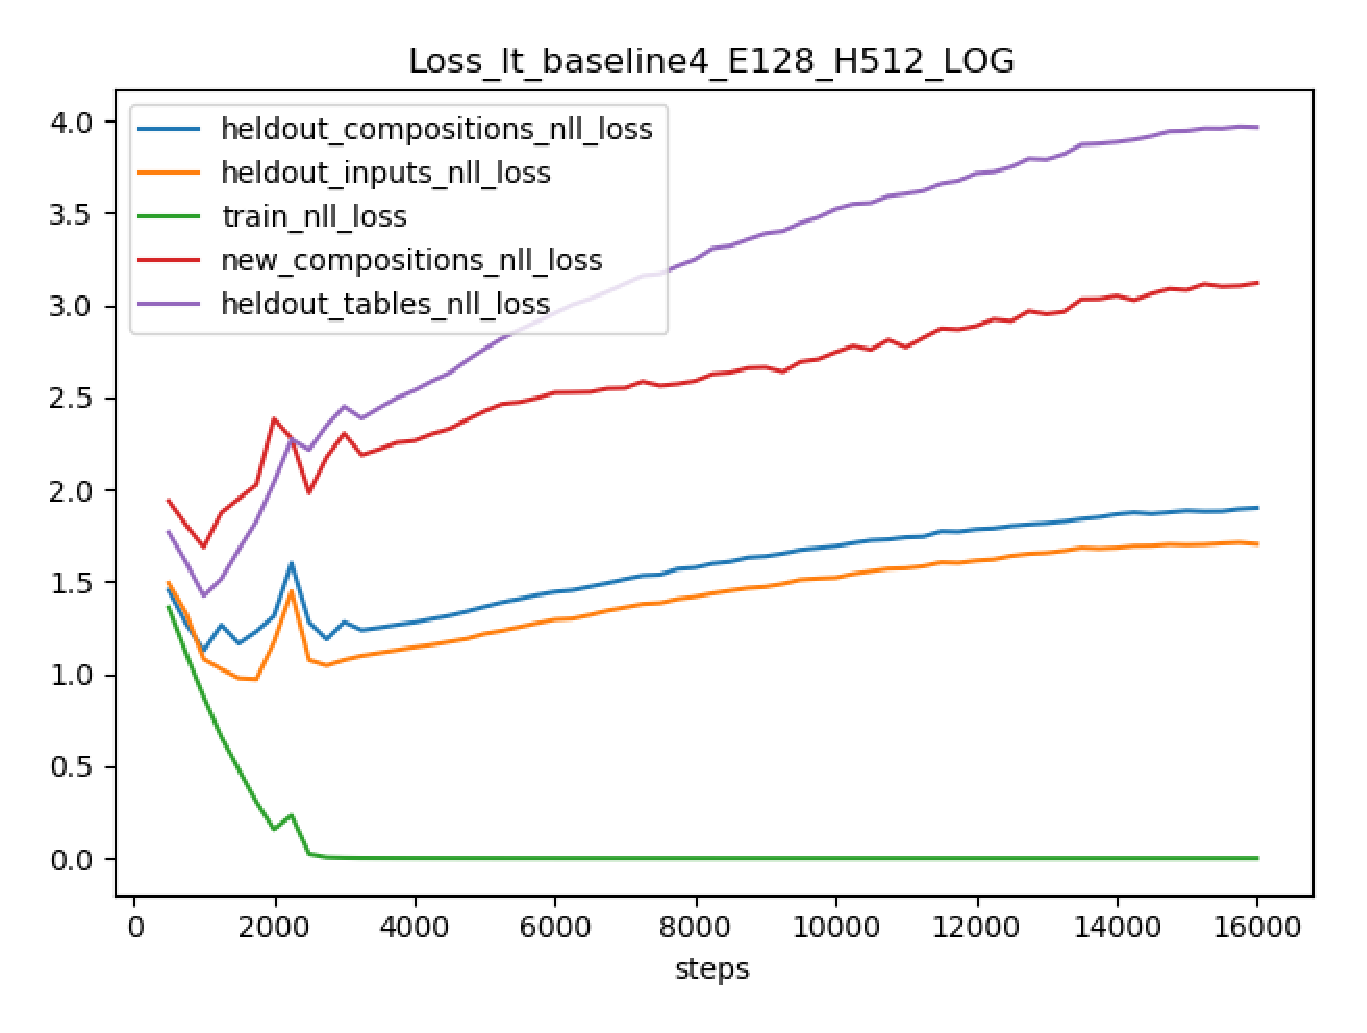
\includegraphics[width=0.95\linewidth]{./figs/lookup/baseline-loss-eps}
		\fi
		\caption{Loss Curves for Baseline} 
		\label{lt_baseline} 
		\vspace{2ex}
	\end{subfigure}%% 
	\begin{subfigure}[b]{0.5\linewidth}
		\centering
		\ifpdf
		\includegraphics[width=0.95\linewidth]{./figs/lookup/learned-loss-pdf}
		\else
		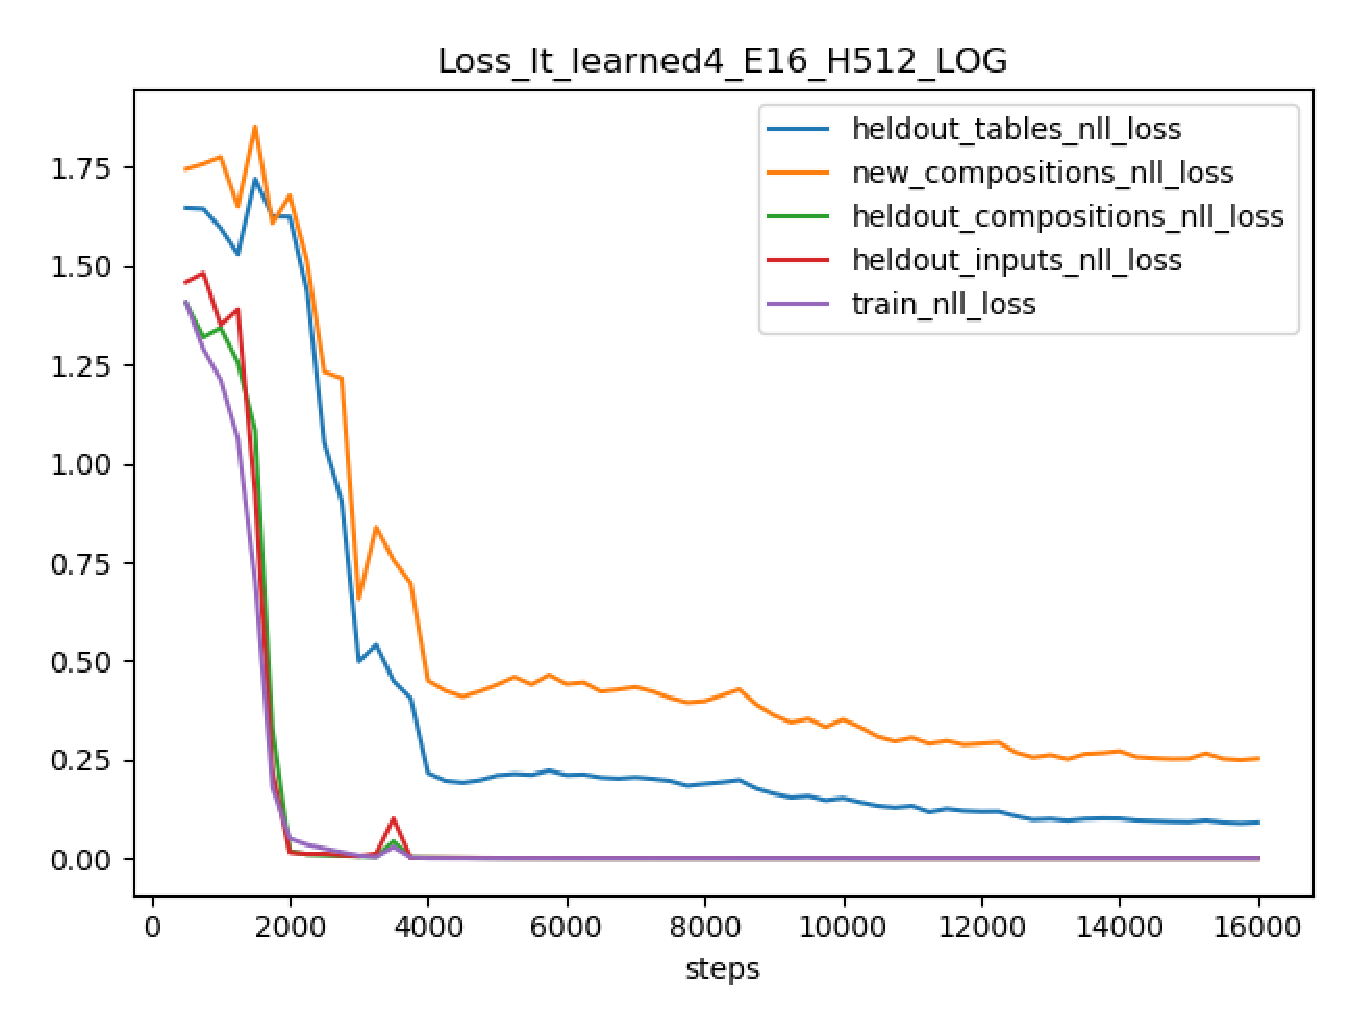
\includegraphics[width=0.95\linewidth]{./figs/lookup/learned-loss-eps}
		\fi 
		\caption{Loss Curves for Learned} 
		\label{lt_learned} 
		\vspace{2ex}
	\end{subfigure}
	\caption{Learning Curves for Lookup Tables}
	\label{lt_learning_curves}
\end{figure}

\begin{figure}
	\begin{minipage}[t]{\textwidth}
		\ifpdf
		\includegraphics[width=\linewidth,keepaspectratio=true]{./figs/lookup/lt-acc-pdf}
		\else
		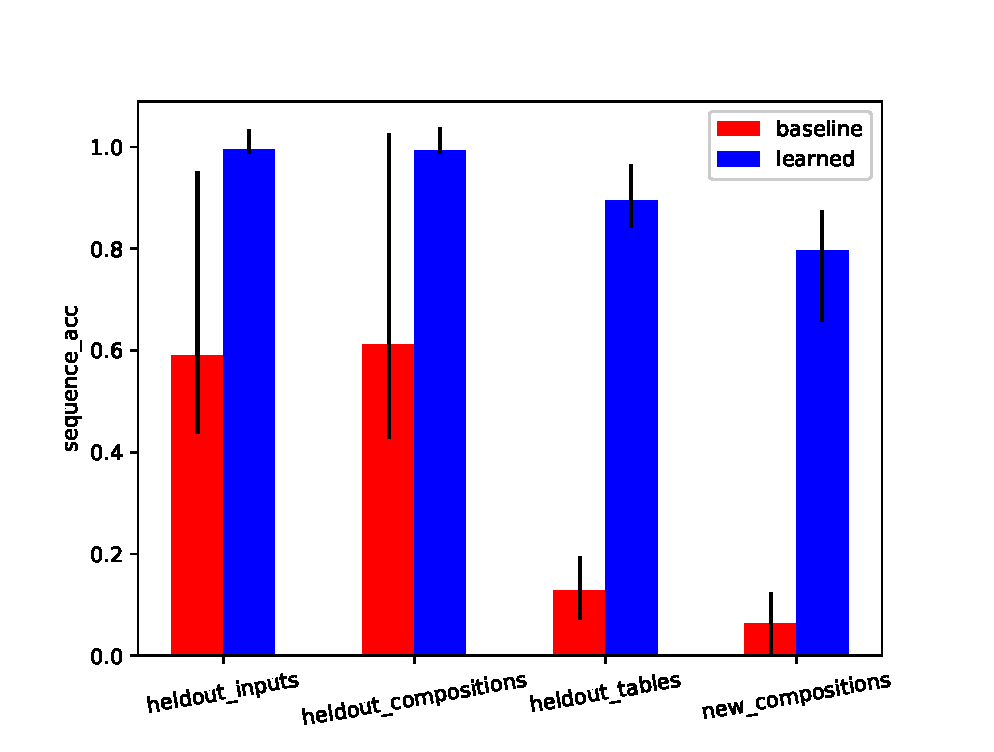
\includegraphics[width=\linewidth,keepaspectratio=true]{./figs/lookup/lt-acc-eps}
		\fi
		\caption{\small Average Sequence Accuracies}
		\label{res:lt-acc}
	\end{minipage}
\end{figure}